\section{Procedure e protocolli}
\subsection{Protocollo di sviluppo del progetto}
\subsubsection{Utilizzo del ticketing}
Le figure che avranno accesso al sistema di \textit{ticketing} sono le seguenti:

\begin{itemize}
\item Il \textit{Responsabile di Progetto} assegnerà i \textit{ticket} di massima importanza cioè quelli correlati allo sviluppo delle attività necessarie all' avanzamento del progetto;
\item Il \textit{Verificatore} potrà assegnare \textit{ticket} allo scopo di segnalare errori di grave entità rilevati durante l'attività di verifica.
\end{itemize}

Di conseguenza i \textit{ticket} sono suddivisi in due macro-categorie:
\begin{itemize}
\item \textit{Ticket} di pianificazione, i quali rappresentano le attività che devono essere svolte per procedere con l'avanzamento del progetto, sono suddivisi in 4 sotto-categorie:
\begin{itemize}
\item \emph{Documento}: che rappresenta una \textit{task} inerente alla redazione di un documento; 
\item \emph{Codice}: che rappresenta una \textit{task} inerente alla stesura di codice;
\item \emph{Verifica}: che rappresenta una \textit{task} inerente all'attività di verifica di un'attività;
\item \emph{Generali}: che rappresenta \textit{tasks} i cui scopi sono svariati ed in genere non ad alta priorità, come ad esempio la ricerca di un determinato \textit{software}.
\end{itemize}
lo svolgimento dell'insieme di tutti i ticket di una \textit{task-list} non porterà alla conclusione della \textit{task-list} stessa, questo poiché è prevista la possibilità di aggiungere durante l'avanzamento del progetto ulteriori \textit{task}, fino a quando il \textit{responsabile di progetto} non ne dichiarerà la conclusione;
\item Ticket di verifica, contenenti gli errori identificati dai \textit{verificatori} a seguito dell'analisi del lavoro svolto da qualche membro del \textit{team}.
\end{itemize}

Ogni membro del \textit{team} sarà tenuto ad utilizzare la barra di avanzamento di stato del \textit{ticket} fornita dall'interfaccia di \textit{TeamWorkPM}, evitando così superflue norme aggiuntive atte a determinare lo stato del \textit{ticket}.

\subsubsection{Creazione di una milestone}
Il \textit{Responsabile di Progetto} dovrà creare una \textit{milestone}, essa indica la data della revisione a cui il gruppo \gruppo{} intende presentarsi, è possibile visualizzare lo stato di avanzamento che tiene conto del numero di \textit{ticket} completati rispetto al numero di \textit{ticket} complessivi.
Per la creazione di una nuova \textit{milestone} il \textit{Responsabile di Progetto} dovrà seguire i seguenti passi:
\begin{enumerate}
\item Aprire il progetto dall'interfaccia \textit{web} di \textit{TeamWorkPM};
\item Posizionarsi sull'opzione: "\emph{Milestones}" ed accedervi;
\item Cliccare sull'opzione: "\emph{Add a new milestone}".
\end{enumerate}

Completati questi passaggi apparirà il seguente \textit{form\ped{G}} (fig 1) che dovrà essere compilato per concludere la creazione della una \textit{milestone}.
\begin{figure}
\centering
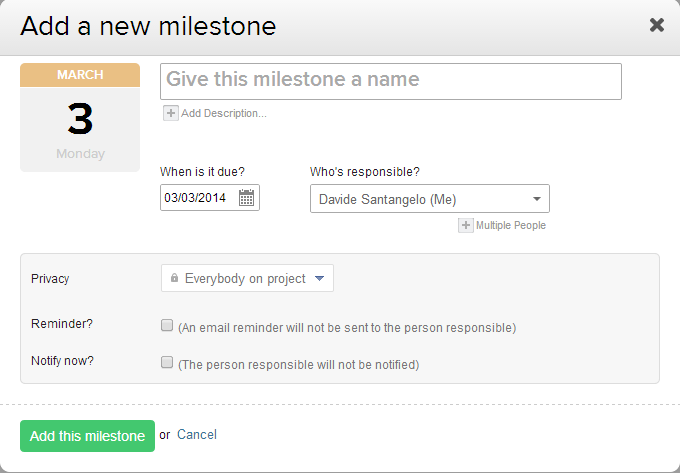
\includegraphics[width=%
\textwidth]{immaginiNDP/Immagine}
\caption[]{Creazione di una milestone.}
\label{fig:Immagine}
\end{figure}

\subsubsection{Procedura di creazione ticket} 
Il \textit{Responsabile di Progetto} dovrà attenersi alla seguente procedura per la creazione di una nuova task-list, ovvero la concretizzazione di un macro-attività e delle sue relative task (ticket). Si ricorda che TeamWorkPM prevede la possibilità di indicare interdipendenze tra task-list.
\begin{enumerate}
\item Dall'interfaccia \textit{web} accedere al progetto \progetto{}, e selezionare dal \textit{menù} principale il comando: \emph{"Task"};
\item Procedere, se necessario, con la creazione di una nuova \textit{task-list} tramite il comando: \emph{"Add task list"};
\item Una volta creata la \textit{task-list} sarà possibile creare i \textit{ticket} (\textit{Task} nel contesto di \textit{TeamWorkPM}) inerenti alla \textit{task-list} scelta.
\end{enumerate}

La struttura di un \textit{ticket} è visualizzabile nella figura 2 di questa sezione.
\begin{figure}
\centering
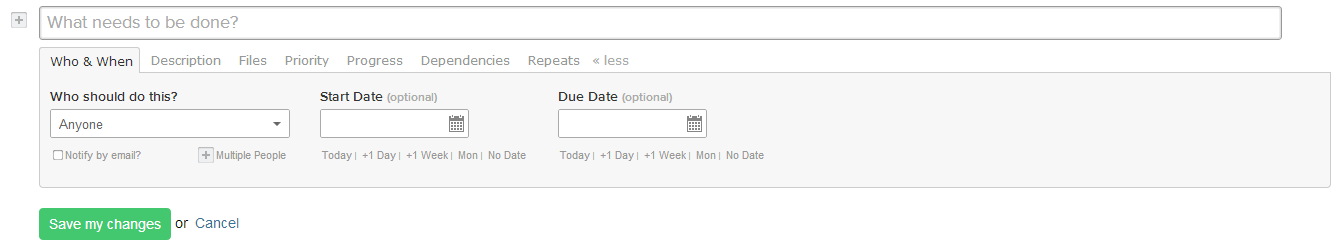
\includegraphics[width=%
\linewidth]{immaginiNDP/creazionetask}
\caption[]{Creazione di un ticket.}
\label{fig:creazionetask}
\end{figure}

Nella task è necessario specificare \textbf{obbligatoriamente}:
\begin{itemize}
\item Il \textbf{Titolo} del \textit{ticket}, dovrà contenere tra parentesi quadre la categoria (per i \textit{ticket} di pianificazione anche la sotto-categoria) di \textit{ticket} di cui si tratta;
\item Il \textbf{Destinatario} del \textit{ticket}, cioè colui a cui è stato assegnato;
\item Le \textbf{Date} di inizio e scadenza del \textit{ticket};
\item Le \textbf{Dipendenze} del \textit{ticket}, che specificano l' eventuale necessità di attendere la terminazione di un insieme di \textit{task} prima di poter svolgere quel determinato compito;
\item Una \textbf{Descrizione} la quale dovrà essere breve e coincisa, ma spiegare efficacemente il lavoro assegnato;
\item La \textbf{Priorità} del \textit{ticket} suddivisa in tre categorie: bassa, media, alta.
\end{itemize}

Compilati i seguenti campi, il \textit{ticket} sarà creato ed inviato regolamentarmene.

\subsubsection{Procedura di terminazione ticket}
Se un \textit{ticket} sarà completato è necessario applicare questa procedura di accertamento:
\begin{enumerate}
\item Il membro del \textit{team} a cui è stato assegnato il \textit{ticket} dovrà spuntare la casella di terminazione su \textit{TeamWorkPM};
\item Durante il controllo giornaliero il \textit{Responsabile di Progetto} controllerà quanto necessario a determinare che il lavoro sia stato effettivamente svolto;
\item Se il lavoro è stato effettivamente svolto, sarà avviato un \textit{ticket} di \emph{Pianificazione} a scopo di verificare il lavoro;
\item Nel caso di irregolare svolgimento del \textit{ticket} o problemi di grave entità, il \textit{Responsabile di Progetto} dovrà applicare la procedura di modifica o riassegnazione del \textit{ticket} presente nel prossimo paragrafo;
\item Nel caso di esito positivo (cioè con regolare svolgimento) il \textit{ticket} sarà concluso ed archiviato, mentre al contempo, qualora fosse necessario, saranno avviati dei \textit{ticket} di \emph{Verifica} per la correzione degli errori non gravi rilevati durante la \textit{Verifica};

\end{enumerate}

\subsubsection{Procedura per la modifica o riassegnazione ticket} 
Durante il suo ciclo di vita un \textit{ticket} per varie ragioni può andare in contro a modifiche, è necessario quindi normare la seguente procedura:
\begin{enumerate}
\item Aprire il progetto dall'interfaccia \textit{web} di \textit{TeamWorkPM};
\item Selezionare il \textit{ticket} di interesse;
\item Selezionare il comando: \emph{"Edit Task"};
\item Aggiungere una descrizione riguardo la modifica effettuata;
\item Avvertire l'interessato che è stata effettuata una modifica inserendo: "(MOD)" sul titolo del \textit{ticket}, e qualora fosse necessario reimpostandone la sua priorità.
\end{enumerate}

\subsection{Protocollo di pianificazione}
Il \textit{responsabile di progetto} per ogni attività indicata nel documento \textit{Piano di Progetto} dovrà creare un nuovo progetto seguendo la procedura qui descritta:

\begin{enumerate}
\item Inserire una milestone\ped{G};
\item Inserire le attività da svolgere;
\item Inserire le rispettive sotto-attività;
\item Calcolare ed inserire i periodi di slack\ped{G} qualora fosse necessario;
\item Creare le risorse;
\item Assegnare le risorse create ad ogni attività;
\item Salvare la baseline\ped{G}.
\end{enumerate}

Sarà decisa a discrezione del \textit{Responsabile di Progetto} per ogni attività la possibilità di assegnare un surplus di ore, queste ore supplementari verranno scelte basandosi sulla criticità dell'attività considerata.

\begin{itemize}
\item Per le attività non critiche non è previsto alcun surplus di ore;
\item Per le attività di media criticità il surplus di ore potrà essere del 15\%;
\item Per le attività di criticità massima il surplus di ore potrà essere del 30\%.
\end{itemize}
